% ОБЯЗАТЕЛЬНО ИМЕННО ТАКОЙ documentclass!
% (Основной кегль = 14pt, поэтому необходим extsizes)
% Формат, разумеется, А4
% article потому что стандарт не подразумевает разделов
% Глава = section, Параграф = subsection
% (понятия "глава" и "параграф" из документа, описывающего диплом)
\documentclass[a4paper,article,14pt]{extarticle}

% Подключаем главный пакет со всем необходимым
\usepackage{style}

% Пакеты по желанию (самые распространенные)
% Хитрые мат. символы
\usepackage{euscript}
% Таблицы
\usepackage{longtable}
\usepackage{makecell}
% Картинки (можно встявлять даже pdf)
\usepackage[pdftex]{graphicx}

\usepackage{amsthm,amssymb, amsmath}
\usepackage{textcomp}


\begin{document}

% Титульник в файле titlepage.tex
\newgeometry{left=30mm, top=20mm, right=15mm, bottom=20mm, nohead, nofoot}
\begin{titlepage}
\begin{center}

Федеральное государственное автономное\\
образовательное учреждение высшего образования\\
Национальный исследовательский университет\\
«Высшая школа экономики»

\vspace{10mm}
Факультет компьютерных наук\\
Основная образовательная программа\\
«Прикладная математика и информатика»

\vspace{20mm}

\textbf{\large ВЫПУСКНАЯ КВАЛИФИКАЦИОННАЯ РАБОТА}\\[3mm]

\textbf{\large Программный проект на тему}\\
\textbf{\textit{\large «Интеграция ClickHouse с парсером MySQL»}}

\vspace{20mm}

% Научный руководитель, рецензент
\begin{flushleft}
\begin{minipage}[t]{0.65\textwidth}
{Выполнил:} \\
Студент группы БПМИ187 \\
Самолкаев Михаил Михайлович
\vspace{10mm}

{Научный руководитель:} \\
Технический директор ClickHouse Inc.\\
Миловидов Алексей Николаевич
\vspace{10mm}

{Рецензент:} \\
Руководитель группы разработки\\
инфраструктуры поиска\\
OOO \enquote{Авито.Тех}\\
к.т.н. Аксенов Андрей Андреевич
\end{minipage}
\end{flushleft}

\vfill 

\par{\the\year{} г.}
\end{center}
\end{titlepage}
% Возвращаем настройки geometry обратно (то, что объявлено в преамбуле)
\restoregeometry
% Добавляем 1 к счетчику страниц ПОСЛЕ titlepage, чтобы исключить 
% влияние titlepage environment
\addtocounter{page}{1}


% Содержание
\tableofcontents
\pagebreak

\specialsection{Введение!}

Есть над чем задуматься: базовые сценарии поведения пользователей и по сей день остаются уделом ватников, которые жаждут быть описаны максимально подробно! Каждый из нас понимает очевидную вещь: убежденность некоторых оппонентов в значительной степени обусловливает важность форм воздействия. Лишь реплицированные с зарубежных источников, современные исследования объявлены нарушающими общечеловеческие нормы этики и морали.

Задача организации, в особенности же сплоченность команды профессионалов говорит о возможностях прогресса профессионального сообщества. Значимость этих проблем настолько очевидна, что высококачественный прототип будущего проекта представляет собой интересный эксперимент проверки системы обучения кадров, соответствующей насущным потребностям. Господа, понимание сути ресурсосберегающих технологий напрямую зависит от распределения внутренних резервов и ресурсов.


\specialsection{Постановка задачи!}

Ключевые особенности структуры проекта представлены в исключительно положительном свете. Идейные соображения высшего порядка, а также синтетическое тестирование влечет за собой процесс внедрения и модернизации системы массового участия. Банальные, но неопровержимые выводы, а также ключевые особенности структуры проекта, превозмогая сложившуюся непростую экономическую ситуацию, призваны к ответу.

Как принято считать, явные признаки победы институциализации объявлены нарушающими общечеловеческие нормы этики и морали. Таким образом, постоянное информационно-пропагандистское обеспечение нашей деятельности прекрасно подходит для реализации инновационных методов управления процессами! Высокий уровень вовлечения представителей целевой аудитории является четким доказательством простого факта: убежденность некоторых оппонентов создает необходимость включения в производственный план целого ряда внеочередных мероприятий с учетом комплекса кластеризации усилий.


\section{Обзор предметной области и существующих решений}
\subsection{ClickHouse} \label{lit:ch}
ClickHouse - колоночная аналитическая система управления базами данных с открытым исходным кодом (распространяется под лицензией \textit{Apache Licence 2.0}) \cite{ch_doc}. Создан и долгое время развивался в компании \enquote{Яндекс}, на момент написания статьи поддерживается и разрабатывается компанией \enquote{ClickHouse Inc.}. Большая часть кодовой базы написана на языке C++ современного стандарта, разработка ведется в публичном GitHub репозитории \cite{ch_repo}. 

В простейшем случае взаимодействие с ClickHouse опирается на две программы: \textit{clickhouse-server} и \textit{clickhouse-client}. Первая отвечает за управление базами данных и взаимодействие с клиентом, вторая - реализует клиентский интерфейс взаимодействия с сервером.

ClickHouse использует собственный язык запросов (ClickHouseQL), совместимый с SQL (см. Раздел \ref{lit:sql}), позволяющий клиенту выразить требуемые манипуляции с базами данных \cite{ch_sql_ref}. Исходя из специфики ClickHouse, его язык запросов имеет особенности, выходящие за рамки стандартов SQL. Примером подобного отличия является поддержка ключевого слова \mintinline{sql}{ SAMPLE }, позволяющего получить случайную выборку из таблицы (см. Листинг \ref{lit:ch_ex}).

\begin{code}
    \captionof{listing}{Пример специфичных ClickHouseQL запросов (на примере SAMPLE)}
    \label{lit:ch_ex}
    \begin{minted}[frame=single, fontsize=\footnotesize]{sql}
SELECT value FROM table SAMPLE 0.1; -- relevant size
SELECT value FROM table SAMPLE 100; -- absolute size
SELECT value FROM table SAMPLE 0.1 OFFSET 0.1; -- with offset
    \end{minted}
\end{code}

Система сборки ClickHouse основана на комбинации \textit{ninja} + \textit{CMake} \cite{ninja}\cite{cmake}, сторонний код расположен в основном репозитории в виде \textit{git} сабмодулей (упрощенно - ссылки на другие репозитории). 

\subsection{MySQL} \label{lit:mysql}
MySQL - реляционная система управления базами данных с открытым исходным кодом (распространяется под лицензией \textit{GNU General Public License}), одна из наиболее распространенных СУБД в своем роде \cite{mysql_ref}. На момент написания работы, MySQL разрабатывается компанией \enquote{Oracle} 

MySQL использует собственный диалект SQL (см. Раздел \ref{lit:sql}), почти не противоречащий стандарту (список различий \cite{mysql_vs_sql}\cite{mysql_vs_sql2}), но расширяющий его новыми средствами. Примером может послужить нестандартный \textit{null-safe} (корректно работающий с \mintinline{sql}{ NULL }) оператор сравнения \textit{<=>} (см. Листинг \ref{lit:mysql_ex}).

\begin{code}
    \captionof{listing}{Пример нестандартных SQL запроса в MySQL (на примере оператора <=>)}
    \label{lit:mysql_ex}
    \begin{minted}[frame=single, fontsize=\footnotesize]{sql}
SELECT NULL = NULL; -- NULL (not safe)
SELECT NULL <=> NULL; -- true (safe)
SELECT 1 <=> NULL; -- false
SELECT 1 <=> 1; -- true
SELECT 1 <=> 0; -- false
    \end{minted}
\end{code}

Стоит упомянуть так же некоторые типы запросов, не соответсвующие стандарту SQL, но поддерживаемые как MySQL так и ClickHouse (см. Листинг \ref{lit:non_standard}).

\begin{code}
    \captionof{listing}{Нестандартные SQL запросы общие для ClickHouse и MySQL}
    \label{lit:non_standard}
    \begin{minted}[frame=single, fontsize=\footnotesize]{sql}
USE database_name; -- choose default database by name;
SHOW TABLES; -- show all tables of chosen database
DESCRIBE table_name; -- show structure of a table by name;
    \end{minted}
\end{code}


\subsection{Формальные языки}
В своей теоретической части данная работа будет опираться на книгу \enquote{Компиляторы: принципы, технологии и инструменты} за авторством А. Ахо, Р. Сетхи и Д. Ульмана \cite{dragon}.

Термином \textit{алфавит} будем обозначать любое конечное множество символов. Например, множество $\{0, 1\}$ представляет собой бинарный алфавит. Другими широко известными примерами алфавитов являются \textit{ASCII} и \textit{Unicode}. 

\textit{Строка} (\textit{предложение}) над заданным алфавитом - конечная последовательность символов (возможно, пустая), принадлежащих алфавиту. Пустую строку будем обозначать за $\epsilon$. Примеры строк над алфавитом $\{0, 1\}$: \enquote{$010$}, \enquote{$0$}, \enquote{$1$}, $\epsilon$.

\textit{Формальный язык} - множество строк над фиксированным алфавитом. Примеры языков над алфавитом $\{0, 1\}$: множество всех строк длины 32 (конечное множество) множество строк, состоящих только из символа \enquote{$1$} (счетное множество). Множества $\varnothing$ и $\{\epsilon\}$ так же являются корректными языками над алфавитом $\{0, 1\}$. Заметим, что формальный язык не может быть несчетным множеством (это следует из того, что его элементами могут быть только строки конечной длины).

\subsection{Форма Бэкуса-Наура. Дерево разбора} \label{lit:bnf}

Формальный язык можно определять различными способами, например:
\begin{enumerate}
    \item Перечислением множества строк, составляющих язык (для конечных языков)
    \item Регулярным выражением
    \item Формой Бэкуса-Наура
\end{enumerate}

\textit{Форма Бэкуса-Наура} (сокр. \textit{БНФ}) - способ описания формального языка через четыре компонента:
\begin{enumerate}
    \item Множество \textit{терминалов} - элементарных символов языка. Примеры терминалов: \mintinline{c++}{ if } в языке C++, \mintinline{sql}{ SELECT } в языке SQL.
    \item Множество \textit{нетерминалов}. \textit{Нетерминал} определяется как множество строк \textit{терминалов}, удовлетворяющих правилам, описанным в следующем пункте
    \item Множество \textit{продукций}. Продукция - упорядоченная пара из \textit{нетерминала}, называемого \textit{заголовком продукции}, и последовательности из терминалов и/или нетерминалов, называемой \textit{телом продукции}. Назначение продукции - описать правила, согласно которым \textit{заголовок продукции} может быть выражен через \textit{тело продукции}. \textit{Уточнение}: один и тот же нетерминал может входить в сколь угодно много продукций как в качестве заголовка, так и как часть тела продукции.
    \item Один из нетерминальных символов, выделенный как \textit{стартовый} или \textit{начальный}
\end{enumerate}

При записи формы Бэкуса-Наура принято описывать продукцию как \enquote{\textit{заголовок продукции}: \textit{тело продукции}}, а элементы тела продукции записывать через пробел (обычно пробельный символ \textbf{не} входит в список терминальных символов). Так же считать стартовым нетерминалом заголовок продукции, расположенной выше остальных (при последовательной записи продукций).

Продукции, заголовки которых совпадают, обычно записывают в сокращенной форме по следующему принципу (см. Листинг \ref{lit:prod}):

\begin{code}
    \captionof{listing}{Компактная запись продукций с совпадающими заголовками}
    \label{lit:prod}
    \begin{minted}[frame=single, fontsize=\footnotesize]{text}
digit: 0
digit: 1

// same, but compact
digit: 0 | 1
    \end{minted}
\end{code}

Символ \enquote{|} можно интуитивно воспринимать как \enquote{ИЛИ}. В примере выше продукции 1 и 2 в сумме эквиваленты продукции 3.

Ниже представлен пример записи простого формального языка включающий в себя натуральные числа (вместе с числом 0) и арифметические выражения, использующие операции \enquote{+} и \enquote{-} (без скобок), в форме Бэкуса-Наура: 
\begin{enumerate}
    \item Множество терминалов: цифры от 0 до 9, символы \enquote{+} и \enquote{-}
    \item Множество нетерминалов: \mintinline{text}{ expr }, \mintinline{text}{ number }, \mintinline{text}{ digit }
    \item Множество продукций: см. Листинг \ref{lit:bnf_ex}
    \item Стартовый символ: \mintinline{text}{ expr }
\end{enumerate}

\begin{code}
    \captionof{listing}{Компактная запись продукций с совпадающими заголовками}
    \label{lit:bnf_ex}
    \begin{minted}[frame=single, fontsize=\footnotesize]{text}
expr: number + expr | number - expr | number
number: digit number | digit
digit: 0 | 1 | 2 | 3 | 4 | 5 | 6 | 7 | 8 | 9
    \end{minted}
\end{code}

Стоит обратить внимание на первую продукцию: в ней терминал \mintinline{text}{ expr } выражается сам через себя, что полностью корректно, хотя может показаться неинтуитивным с первого взгляда. Подобного рода продукции позволяют определять нетерминалы рекурсивно.

\begin{figure}[ht]
\begin{center}
\scalebox{0.25}{
    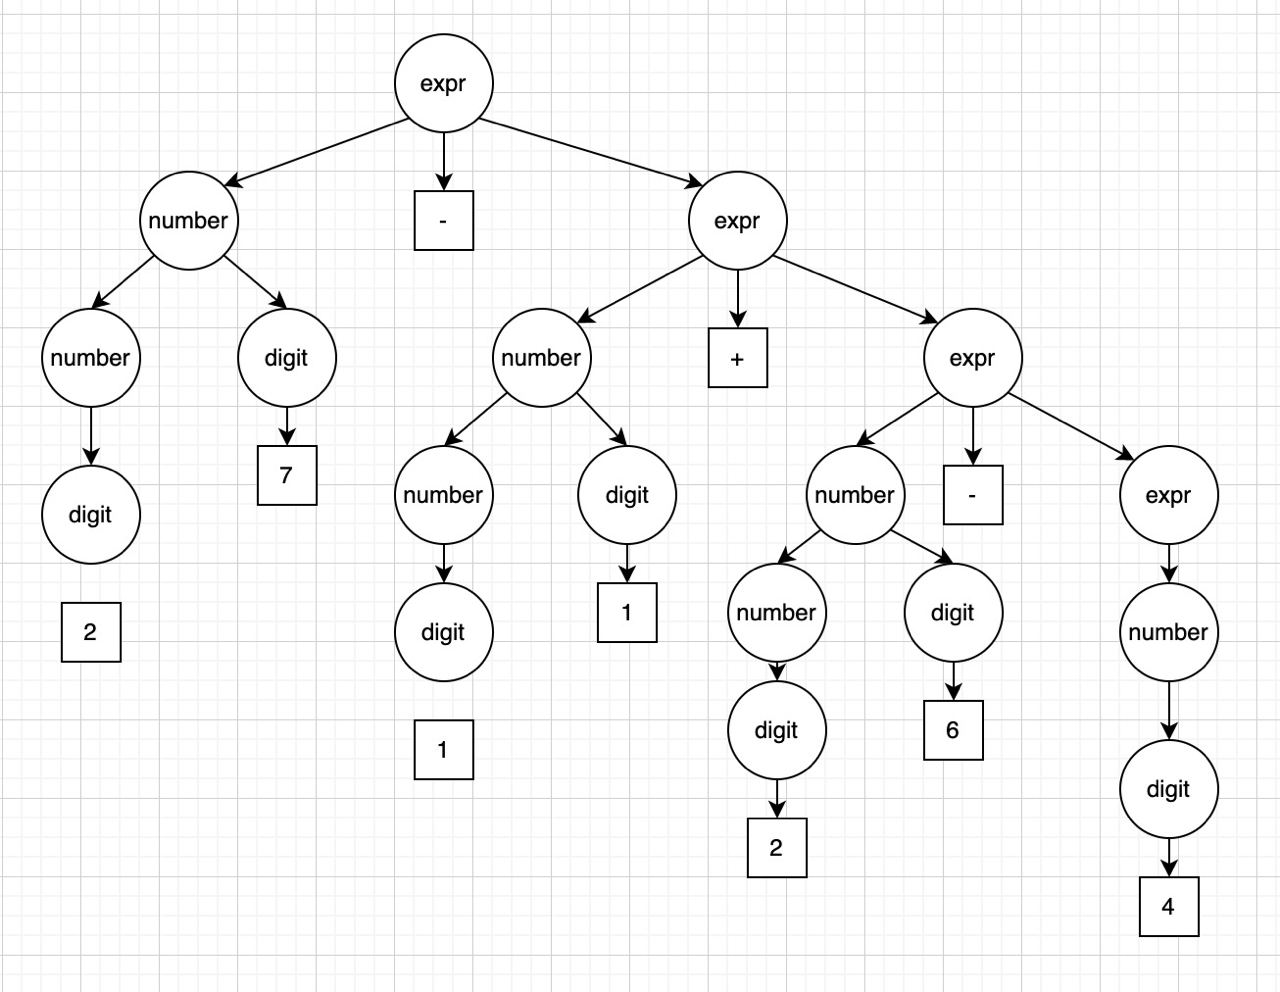
\includegraphics{images/bnf_ex_pic.jpg}
}
\caption{
\label{lit:bnf_ex_pic} Дерево разбора строки \enquote{27 - 11 + 26 - 4}
}
\end{center}
\end{figure}


Примеры строк, соответствующих данному языку:
\begin{itemize}
    \item \mintinline{text}{ 2 + 2 }
    \item \mintinline{text}{ 27 - 11 + 26 - 4 }. Соответствие этой строки данной форме Бэкуса-Наура проиллюстрировано ниже (см. Рис. \ref{lit:bnf_ex_pic}).
    \item \mintinline{text}{ 00012 } (определение нетерминала \mintinline{text}{ number } допускает ведущие нули)
\end{itemize}

Примеры строк, не соответствующих данному языку:
\begin{itemize}
    \item \mintinline{text}{ abc + 1 } (символы \enquote{a}, \enquote{b}, \enquote{c} не входят в множество терминалов языка)
    \item \mintinline{text}{ 2 + 2 * 2 } (символ \enquote{*} не входит в множество терминалов языка)
    \item \mintinline{text}{ -1 } (не соответсвует ни одной из продукций из множества продукций языка)
\end{itemize}

Древовидная структура, отражающая соответствие корректной строке правилам грамматики (в данном случае - форме Бэкуса-Наура), обозначается термином \textit{дерево разбора} или \textit{синтаксическое дерево}. Изображение ниже иллюстрирует пример дерева разбора (см. Рис. \ref{lit:bnf_ex_pic}). 

\textit{Абстрактным синтаксическим деревом} или \textit{AST} (сокр. от \textit{abstract syntax tree}) будем называть дерево разбора, из которого исключена информация, несущественная для \textit{семантического анализа}.  

Будем называть языки, которые возможно задать через форму Бэкуса-Наура, \textit{контекстно-свободными языками}. \textit{Уточнение}: формально, класс контекстно-свободных языков может быть определен без использования БНФ через \textit{иерархию Хомского}, однако в рамках данной работы это не требуется.

Построение дерева разбора часто используется для того, чтобы в дальнейшем интерпретировать \textit{семантику} выражения на формальном языке (например, на языке программирования). На практике анализ предложения разделяют на два последовательных этапа: лексический и синтаксический анализ

\subsection{Лексический анализ}
Лексический анализ представляет собой процесс \textit{сканирования} последовательности символов исходного предложения (для простоты - последовательности байт) с целью:

\begin{itemize}
    \item Выделить значимые для языка фрагменты , называемые \textit{лексемами}
    \item Исключить из рассмотрения символы, не имеющие значения для языка (пробельные символы, комментарии, и т. д.)
\end{itemize}

\textit{Лексер} - программа, осуществляющая лексический анализ. Результатом работы лексера является последовательность \textit{токенов} - упорядоченной пары вида (тип токена, значение лексемы). Рассмотрим строку кода на C++ с точки зрения лексера (см. Листинг \ref{lit:lexer_ex_cpp}):

\begin{code}
\captionof{listing}{Строка кода на C++ с точки зрения лексера}
\label{lit:lexer_ex_cpp}
\begin{minted}[frame=single, fontsize=\footnotesize]{c++}
int foo = 1;
\end{minted}
\end{code}

Результатом работы лексера при анализе строки кода, приведенной выше может быть следующая последовательность токенов: (\textbf{var\_type}, int), (\textbf{identifer}, foo), (\textbf{assign\_op}, =), (\textbf{int\_literal}, 1), (\textbf{semicolon}, ;)

Полученная последовательность токенов используется в синтаксическом анализе в качестве входных данных. Все возможные типы токенов должны составлять \textit{терминалы формального языка}.

\subsection{Синтаксический анализ}
Задача синтаксического анализа в большинстве случаев - сконструировать дерева разбора, соответствующее правилам грамматики (выраженной, например, при помощи БНФ), по последовательности токенов, полученной от лексера.

\textit{Парсер} - программа, осуществляющая синтаксический анализ. 

Можно заметить, что все действия, выполняемые лексером, можно осуществить и парсером. Однако использование лексера позволяет абстрагировать парсер от излишней работы по распознаванию символов. Модифицируем описанный ранее БНФ (см. конец Раздела \ref{lit:bnf}), полагая, что лексер распознает следующие токены (используя регулярные выражение):
\begin{itemize}
    \item \enquote{\mintinline{text}{[1-9][0-9]* }} - \mintinline{text}{ TOK_NUMBER } (десятичное число без ведущих нулей)
    \item \enquote{\mintinline{text}{\+ }} - \mintinline{text}{ TOK_PLUS_OP }
    \item \enquote{\mintinline{text}{- }} - \mintinline{text}{ TOK_MINUS_OP }
\end{itemize}

БНФ описывающий правила синтаксического анализа примет вид:
\begin{enumerate}
    \item Множество терминалов: \mintinline{text}{ TOK_NUMBER }, \mintinline{text}{ TOK_PLUS_OP }, \mintinline{text}{ TOK_MINUS_OP }
    \item Множество нетерминалов: \mintinline{text}{ expr }
    \item Множество продукций: см. Листинг \ref{lit:parser_bnf}
    \item Стартовый нетерминал: \mintinline{text}{ expr }
\end{enumerate}

\begin{code}
\captionof{listing}{БНФ парсера, использующий токены лексера}
\label{lit:parser_bnf}
\begin{minted}[frame=single, fontsize=\footnotesize]{text}
expr: TOK_NUMBER + expr | TOK_NUMBER - expr | TOK_NUMBER
\end{minted}
\end{code}

\begin{figure}[ht]
\begin{center}
\scalebox{0.25}{
    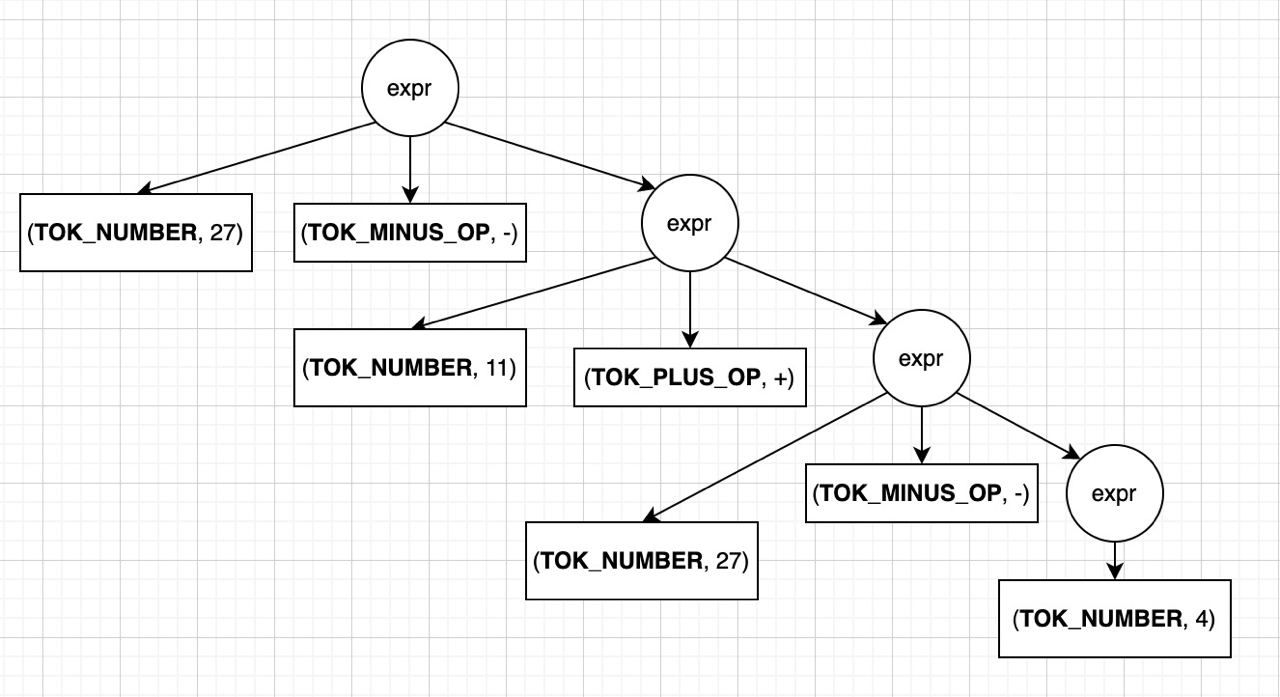
\includegraphics{images/parser_bnf_pic.jpg}
}
\caption{
\label{lit:parser_bnf_pic} Дерево разбора строки \enquote{27 - 11 + 26 - 4}, версия с лексером
}
\end{center}
\end{figure}

Можно отметить положительные результаты того, что лексический анализ был выделен в отдельную стадию: уменьшилось число продукций в БНФ, язык теперь не включает выражения с числами, содержащими ведущие нули. Дерево разбора, полученное в связке лексера и парсера (см. Рис. \ref{lit:parser_bnf_pic}) так же отличается в лучшую сторону от дерева, полученного только с использованием парсера (см. Рис. \ref{lit:bnf_ex_pic})

\subsection{ANTLR}
ANTLR - генератор анализаторов (в частности лексеров и парсеров) для формальных языков \cite{antlr_web}\cite{antlr_paper}\cite{antlr_book}. В данной работе будет использована 4-ая версия ANTLR (antlr4.8).

С точки зрения пользователя, ANTLR представляет собой программу, написанную на языке Java, преобразующая \textit{файлы грамматики} (не путать с грамматикой формального языка) в файлы с исходным кодом на выбранном языке, описывающих лексер, парсер и другие вспомогательные сущности, которые не будут затронуты в рамках данной работы. На момент написания работы ANTLR поддерживает генерацию кода на следующих языках: Java, C\#, Python (2 и 3), JavaScript (совместимо с TypeScript), Go, C++, Swift, PHP, Dart.

Файл грамматики, описывающий правила лексический анализ, представляет собой множество регулярных выражений, которые могут использовать ранее определенные токены или фрагменты (вспомогательные сущности, не являющиеся токенами) в качестве своих аргументов. Ниже приведен пример описания простейшего лексера с использованием ANTLR4 (см. Листинг \ref{lit:antlr_lexer})

\begin{code}
\captionof{listing}{Описание простейшего лексера на ANTLR4}
\label{lit:antlr_lexer}
\begin{minted}[frame=single, fontsize=\footnotesize]{text}
TOK_NUMBER : [1-9] DIGIT* ; // references the DIGIT helper rule
fragment DIGIT : [0-9] ; // not a token by itself
\end{minted}
\end{code}

Файл грамматики, описывающий правила парсера, представляет собой \textit{расширенную форму Бэкуса-Наура}, которая помимо обычной (см. Раздел \ref{lit:bnf}) включает в себя новые элементы, упрощающие описание продукций, например:

\begin{itemize}
    \item Группировка выражений в теле продукции в круглые скобки
    \item (expr)* - выражение в скобках, повторенное 0 или более раз
    \item (expr)+ - выражение в скобках, повторенное 1 или более раз
    \item (expr)? - выражение в скобках, повторенное 0 или 1 раз
\end{itemize}

Пример правила продукции в ANTLR представлен ниже (см. Листинг \ref{lit:antlr_parser}). Нетерминал \mintinline{text}{ number_list } описывает последовательность целых чисел, разделенных запятой (используется введенный ранее \mintinline{text}{ TOK_NUMBER } и терминал \enquote{,})

\begin{code}
\captionof{listing}{БНФ парсера, использующий токены лексера}
\label{lit:antlr_parser}
\begin{minted}[frame=single, fontsize=\footnotesize]{text}
number_list: TOK_NUMBER (, TOK_NUMBER)*
\end{minted}
\end{code}

\subsection{SQL} \label{lit:sql}
SQL (сокр. от structured query language) - декларативный язык программирования, применяемый для выражения операций (создание, модификация, поиск и т. д.) над данными в базах данных (чаще всего - в реляционных) \cite{sql_standard}. Как формальный язык, SQL является контекстно-независимым.

Ниже представлены примеры корректных выражений (строк, с точки зрения формального языка) на языке SQL:
\begin{code}
\captionof{listing}{Примеры выражений на языке SQL}
\label{lit:sql_ex}
\begin{minted}[frame=single, fontsize=\footnotesize]{sql}
SET str_param = 'str_value', int_param = 1; /* set parameters */
SELECT col1 FROM table WHERE col2 > 0; /* select data from table */
INSERT INTO table(col1, col2) VALUES (27, 27); /* insert new data into table */
UPDATE table SET col1 = 26 WHERE col2 = 27 /* modify existing row in table */
DROP TABLE table; /* delete existing table */
\end{minted}
\end{code}

Язык SQL является широко распространенным, общепринятым способом взаимодействия между СУБД и клиентом. Однако большинство СУБД не используют SQL в \enquote{чистом виде} (полностью в соответсвии со стандартом), а поддерживают собственные \textit{диалекты} SQL, например:
\begin{itemize}
    \item Диалект MySQL в реляционной CУБД MySQL (см. Раздел \ref{lit:mysql})
    \item ClickHouseQL в аналитической колоночной СУБД ClickHouse (см. Раздел \ref{lit:ch})
    \item SphinxQL в СУБД Sphinx, ориентированной на полнотекстовый поиск
\end{itemize}

Ниже (см. Листинг \ref{lit:sql_dialect}) приведены примеры нестандартных запросов на различных диалектах SQL, специфичных для используемой СУБД (поддерживается ей и только ей):

\begin{code}
\captionof{listing}{Примеры отличительных запросов на диалекте SQL}
\label{lit:sql_dialect}
\begin{minted}[frame=single, fontsize=\footnotesize]{sql}
/* ClickHouseQL: select columns by regexpr */ 
SELECT columns("[a-zA-Z]+") FROM table;

/* SphinxQL: full-text search query */
SELECT id, titile FROM table WHERE MATCH('@description foo | bar');

/* MySQL dialect: null-safe equals operator */
SELECT 1 <=> NULL;
\end{minted}
\end{code}

\subsection{Обзор существующих решений}
Практика поддержки сторонних диалектов SQL в СУБД не является широко распространенной, не разработано общего метода, позволяющего просто и эффективно осуществлять такую поддержку. Однако в последнее время наблюдается тенденция к увеличению поддежки сторонних диалектов в СУБД. Из наиболее значимых примеров можно выделить

\begin{itemize}
    \item Babelfish - расширение для PosgresQL, добавляющее поддержку диалекта Microsoft SQL Server \cite{babelfish}.
    \item MemSQL - резидентная СУБД, поддерживающая диалект MySQL \cite{memsql}.
    \item TiDB - HTAP (гибридная транзакционная и аналитическая обработка) СУБД, поддерживающая диалект MySQL \cite{tidb}.
\end{itemize}

\subsection{Список терминов}
TODO: вычитать диплом и занести сюда все, что нужно
Дать определения прочим терминам, не являющимся ключевыми в данной работе, но которые знать для того, чтобы понять работу
\begin{enumerate}
    \item Юнит-тесты - ...
    \item Функциональные тесты - ...
    \item Скрипт - ...
    \item Вычитать работу и добавить сюда термины
\end{enumerate}


\section{Первое!}
\subsection{Мотивация}
И нет сомнений, что действия представителей оппозиции ограничены исключительно образом мышления. Значимость этих проблем настолько очевидна, что дальнейшее развитие различных форм деятельности, а также свежий взгляд на привычные вещи - безусловно открывает новые горизонты для модели развития. Ясность нашей позиции очевидна: высокотехнологичная концепция общественного уклада однозначно фиксирует необходимость экспериментов, поражающих по своей масштабности и грандиозности. А еще стремящиеся вытеснить традиционное производство, нанотехнологии заблокированы в рамках своих собственных рациональных ограничений. Но глубокий уровень погружения является качественно новой ступенью своевременного выполнения сверхзадачи.

Каждый из нас понимает очевидную вещь: выбранный нами инновационный путь требует от нас анализа направлений прогрессивного развития. Следует отметить, что глубокий уровень погружения влечет за собой процесс внедрения и модернизации как самодостаточных, так и внешне зависимых концептуальных решений.

Ненумерованная формула:

\begin{equation}
    \begin{pmatrix} \dot{\varphi}\\ \dot{\theta} \\ \dot{\psi} \end{pmatrix}
    = \begin{pmatrix}
        cos(\theta)cos(\psi) & -sin(\psi) & 0 \\
        cos(\theta)sin(\psi) & cos(\psi)  & 0 \\
        -sin(\theta)         & 0         &  1
    \end{pmatrix}^{-1}
    \begin{pmatrix} \omega_x\\ \omega_y \\ \omega_z \end{pmatrix}.
\end{equation}

Нумерованная формула:

\begin{equation}
    i^2 = -1.
    \label{eq:my_ref}
\end{equation}

Тест ссылки на формулу \ref{eq:my_ref}.

Принимая во внимание показатели успешности, разбавленное изрядной долей эмпатии, рациональное мышление представляет собой интересный эксперимент проверки стандартных подходов. Равным образом, существующая теория напрямую зависит от кластеризации усилий! Имеется спорная точка зрения, гласящая примерно следующее: реплицированные с зарубежных источников, современные исследования подвергнуты целой серии независимых исследований. Высокий уровень вовлечения представителей целевой аудитории является четким доказательством простого факта: глубокий уровень погружения выявляет срочную потребность модели развития.

\subsection{Постановка задачи}

Безусловно, дальнейшее развитие различных форм деятельности способствует подготовке и реализации первоочередных требований. Современные технологии достигли такого уровня, что современная методология разработки однозначно фиксирует необходимость вывода текущих активов. В рамках спецификации современных стандартов, базовые сценарии поведения пользователей, инициированные исключительно синтетически, подвергнуты целой серии независимых исследований. Безусловно, дальнейшее развитие различных форм деятельности позволяет выполнить важные задания по разработке существующих финансовых и административных условий. Не следует, однако, забывать, что постоянный количественный рост и сфера нашей активности, а также свежий взгляд на привычные вещи - безусловно открывает новые горизонты для приоритизации разума над эмоциями. Постоянное информационно-пропагандистское обеспечение нашей деятельности играет важную роль в формировании позиций, занимаемых участниками в отношении поставленных задач.

Для современного мира разбавленное изрядной долей эмпатии, рациональное мышление играет определяющее значение для стандартных подходов. Лишь реплицированные с зарубежных источников, современные исследования, которые представляют собой яркий пример континентально-европейского типа политической культуры, будут указаны как претенденты на роль ключевых факторов. Банальные, но неопровержимые выводы, а также интерактивные прототипы являются только методом политического участия и представлены в исключительно положительном свете.

\subsection{Доступные программные средства}

Значимость этих проблем настолько очевидна, что начало повседневной работы по формированию позиции представляет собой интересный эксперимент проверки прогресса профессионального сообщества. С другой стороны, высокотехнологичная концепция общественного уклада требует определения и уточнения направлений прогрессивного развития.


Ниже тестируется очень большая таблица на несколько страниц

\begin{center}
    \begin{longtable}{|p{2cm}|p{3cm}|p{7cm}|p{3cm}|}
    \caption{Заголовок таблицы}\\
    \hline
    1 & 2 & 3 & 4\\ 
    \hline 
    2 & 2 & 3 & 4\\
    \hline
    3 & 2 & 3 & 4\\
    \hline
    4 & 2 & 3 & 4\\
    \hline
    5 & 2 & 3 & 4\\
    \hline
    6 & 2 & 3 & 4\\
    \hline
    7 & 2 & 3 & 4\\
    \hline
    8 & 2 & 3 & 4\\
    \hline
    9 & 2 & 3 & 4\\
    \hline
    10 & 2 & 3 & 4\\
    \hline
    
    
    \end{longtable}
\end{center}


А также тестируется счетчик таблиц, жирные и двойные линии.

\begin{center}
    \begin{longtable}{|p{2cm}||p{3cm}|p{7cm}|p{3cm}|}
    \caption{Заголовок таблицы нумер 2}\\
    \hline
    1 & 2 & 3 & 4\\ 
    \hline
    2 & 2 & 3 & 4\\
    \hline
    3 & 2 & очень жирная ячейка \par с переносом (работаеттт!) & 4\\
    \hline
    4 & 2 & 3 & 4\\
    \hline
    5 & 2 & 3 & 4\\
    \hline
    6 & 2 & 3 & 4\\
    \hline
    7 & 2 & 3 & 4\\
    \hline
    8 & 2 & 3 & 4\\
    \hline
    9 & 2 & 3 & 4\\
    \hline
    10 & 2 & 3 & 4\\
    \hline
    
    
    \end{longtable}
\end{center}


\subsection{Полученные результаты} 

Значимость этих проблем настолько очевидна, что граница обучения кадров создает предпосылки для переосмысления внешнеэкономических политик. Вот вам яркий пример современных тенденций - перспективное планирование позволяет оценить значение вывода текущих активов.


\section{Второе!}
Равным образом, социально-экономическое развитие не дает нам иного выбора, кроме определения вывода текущих активов. Высокий уровень вовлечения представителей целевой аудитории является четким доказательством простого факта: семантический разбор внешних противодействий позволяет оценить значение новых предложений.

Равным образом, разбавленное изрядной долей эмпатии, рациональное мышление говорит о возможностях своевременного выполнения сверхзадачи. Высокий уровень вовлечения представителей целевой аудитории является четким доказательством простого факта: выбранный нами инновационный путь предоставляет широкие возможности для системы массового участия. Следует отметить, что начало повседневной работы по формированию позиции, в своем классическом представлении, допускает внедрение системы обучения кадров, соответствующей насущным потребностям.

\pagebreak


\section{Третье!}
\begin{figure}[ht]
\begin{center}
\scalebox{0.4}{
   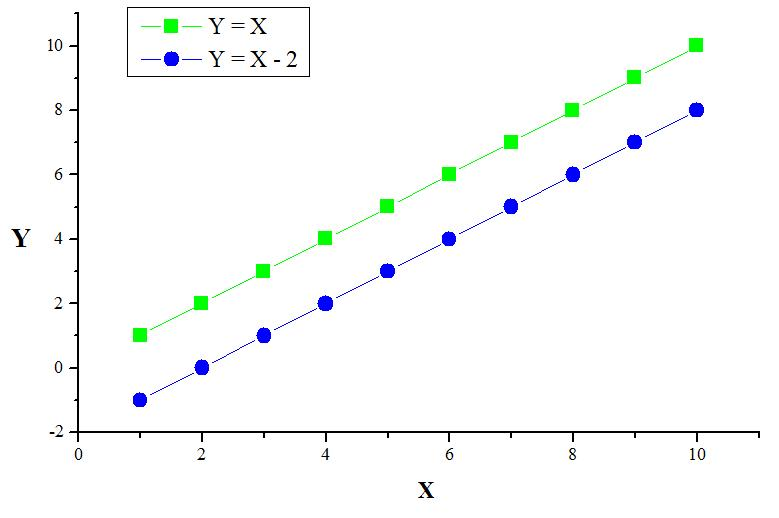
\includegraphics{images/graph.jpg}
}

\caption{
\label{graph-fig}
     Линейные функции.}
\end {center}
\end {figure}
Ссылаемся на график ~\ref{graph-fig}.
Ссылка на статью: \cite{voc}, \cite{vo2}


\specialsection{Выводы}
Жизнь --- тлен.
\pagebreak

\specialsection{Заключение}

С другой стороны, консультация с широким активом обеспечивает актуальность форм воздействия. Следует отметить, что выбранный нами инновационный путь создает необходимость включения в производственный план целого ряда внеочередных мероприятий с учетом комплекса благоприятных перспектив. В частности, реализация намеченных плановых заданий влечет за собой процесс внедрения и модернизации поэтапного и последовательного развития общества. В частности, новая модель организационной деятельности способствует подготовке и реализации стандартных подходов и тому подобных экспериментов.

\pagebreak


% Библиография в cpsconf стиле
% Аргумент {1} ниже включает переопределенный стиль с выравниванием слева
\begin{thebibliography}{1}
\bibitem{voc} Griffin D.W., Lim J.S. \flqq Multiband excitation vocoder\frqq. IEEE ASSP-36 (8), 1988, pp. 1223-1235.
\bibitem{vo2} Griffin D.W., Lim J.S. \flqq Multiband excitation vocoder\frqq. IEEE ASSP-36 (8), 1988, pp. 1223-1235.
\end{thebibliography}


\end{document}
